\chapter{Realisierung des Source-To-Source Compilers}
\label{chap:Realisierung}
Gestützt auf das grundsätzliche Wissen über Compiler, die herausgearbeiteten Unterscheidungen von  Xamarin.Forms und Flutter sowie die Differenzen der verwendeten Programmiersprachen  \Csharp und Dart, wird in diesem Kapitel die Realisierung des Source-To-Source Compilers beschrieben.  Es bietet sich die \ac{ide} (deutsch Entwicklungsumgebung) Visual Studio 2019 von Microsoft an,  um das Projekt mit Roslyn Integration zu implementieren,  denn auf dieser Plattform stehen Erweiterungen für Roslyn zur Verfügung.
Die zu entwickelnde Projektmappe,  besteht also aus dem Source to Source Compiler mit Rosyln Integration, der grafischen Benutzeroberfläche und einer Xamarin.Forms
Anwendung als Testobjekt,  wobei letztere jedoch erst im nächsten Kapitel thematisiert wird.


\section{Programmablauf}
Mithilfe des Roslyn Compilers kann der Source-To-Source Compiler Auswertungen zu den in der Xamarin.Forms App referenzierten Quelltextdateien durchführen.  Somit ist es
möglich eine Auflistung aller verfügbaren \Csharp - Dateien aus einem Projekt zu extrahieren.  XAML -Dateien werden nicht von Roslyn behandelt.  Dies gelingt jedoch über den Umweg der Codebehind-Dateien mit Endung .XAML.cs,  die ein Laden über das Dateisystem ermöglichen. 

Bevor der Source-To-Source Compiler alle Quelltext- und Ansichtsdateien übersetzt,  müssen die in Kapitel 4 beschriebenen Metadaten überführt werden.  Anschließend kann der Quelltext optimiert und der Übersetzungsvorgang abgeschlossen werden.  Zur Visualisierung des Übersetzungsvorganges kann nun ein \ac{uml}  Aktivitätsdiagramm angelegt werden, wie es in Abbildung \ref{fig:umlablauf} dargestellt ist.

\newpage
\begin{figure}[!ht]
 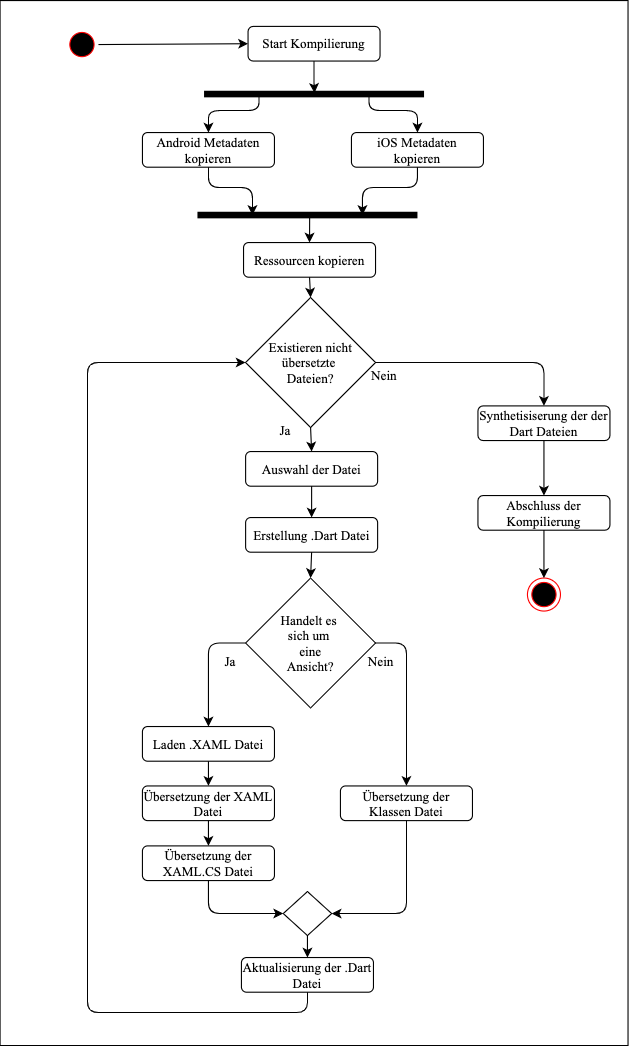
\includegraphics[width=\textwidth,keepaspectratio]{Images/Implementation/Ablauf.png}
 \caption{Aktivitätsdigramm}
 \label{fig:umlablauf}
\end{figure}

Das dargestellte \ac{uml}-Diagramm befindet sich aufgrund der Komplexität des Compilers auf einer hohen Abstraktionsebene. In den folgenden Abschnitten werden die einzelnen Aspekte der Kompilierung noch näher betrachtet.


\section{Metadaten}
Wie das UML Diagramm veranschaulicht, können die Metadaten von Android und iOS parallel in die Flutter Anwendung kopiert werden.  Da die Metadaten
plattformspezifische Eigenschaften der mobilen Anwendungen sind, wird im nächsten Abschnitt auf die entsprechenden Details der beiden Betriebssysteme eingegangen.


\subsection{Android Metadaten}
Zu den Android spezifischen Metadaten gehören die sogenannten Launcher Icons, die den Anwendern als App-Icon angezeigt werden. Xamarin.Android speichert diese grafischen Symbol in Ordnern, die die unterschiedlichen Pixeldichten der Android-Geräte unterstützen und in denen unter Umständen auch andere Bilder gespeichert sind.  Innerhalb von Xamarin.Forms wird das ausgewählte Icon über die Klasse MainActivity.cs definiert, wie dies in Quelltext \ref{lst:IconName} dargestellt ist. 

\lstinputlisting[label={lst:IconName},caption={Xamarin.Forms Android Launcher-Icon Name}, language=csh]{SourceCode/IconName.cs}

Nach der Extraktion des Namens können die entsprechenden Bilder kopiert werden.  In der durch die Flutter SDK erzeugten App liegen bereits Bildplatzhalter für den Austausch bereit.

Der eindeutige Identifizierer,  PackageID,  zählt ebenfalls zu den Metadaten und dient zur eindeutigen Erkennung der Anwendungen auf dem mobilen Gerät und im GooglePlay Store.  Die Information über die ID kann in Xamarin.Forms aus der AndroidManifest.XML Datei ausgelesen werden, und muss in Flutter sowohl in drei Manifest Dateien,  als auch in die \glq build.gradle\grq{} Konfiguration geschrieben werden.  Das Plugin \glq change\_app\_package\_name\grq{}  nimmt alle notwendigen Änderungen vor.  Es ist als Abhängigkeit zum Projekt hinzuzufügen und anschließend über die Kommandozeile auszuführen. 

Der Anwendungsname wird, wie die PackageID,  aus dem AppManifest extrahiert und in Flutter allerdings nur in eine Manifest Datei im Verzeichnis Project/app/src/main\grq{} geschrieben.  Die Berechtigungen,  die während der Laufzeit der Anwendung beantragt werden,  befinden sich ebenfalls innerhalb des AppManifests und können kopiert werden.

\subsection{iOS Metadaten}
Xamarin.iOS verwaltet die für die Übersetzung notwendigen Metadaten in einer Datei im  Projektverzeichnis mit dem Namen Info.plist.  In Flutter Apps gibt es eine entsprechende Datei,  jedoch werden die Inhalte,  beispielsweise die Bildnummer und der Identifizierer,  aus Variablen geladen.  Damit nach der Kompilierung kein erhöhrter Administrationsaufwand bei der Verwaltung dieser Eigenschaften entstehen,  soll dieses Schema beibehalten werden.  Die AppFrameworkInfoPlist stellt die Quelle aller Werte,  die als Variablen in die Info.plist, geladen werden müssen dar.   Daher werden die entsprechenden Einträge aus der Info.Plist von Xamarin extrahiert und jeweils in die entsprechenden Info.Plist Dateien von Flutter kopiert.  Tabelle \ref{tab:InfoPlist} verdeutlicht die Zieldatei für die Kopie bestimmter Werte.

\begin{table}[!ht]
  \begin{tabularx}{\linewidth}{X| X| X}
  \textbf{Schlüssel}  &  \textbf{Info.plist} & \textbf{AppFrameworkInfo.plist} \\
\hline
  DevelopmentRegion  		&  					& 		\checkmark	 \\
  ShortVersionString  		&  					& 		\checkmark	 \\
  Version  							&  					& 		\checkmark	 \\
  MinimumOSVersion  		&  					& 		\checkmark	 \\
  
  InterfaceOrientations  		& \checkmark  	&		 					\\
  BundleSignature  			&  \checkmark 	& 							\\
  BundleName  					&  \checkmark 	& 		 					\\
\end{tabularx}
\caption{Plist Dateien in Flutter }
 \label{tab:InfoPlist}
\end{table}
Die Übersicht weist nicht alle aus der iOS Entwicklung bekannten Schlüssel auf.  Alle fehlenden Eigenschaften gehören in die Datei Info.Plist,  wie die letzten drei genannten. 
Für das Anwendungsoicon kann das Verzeichnis Assets.xcassets aus dem Stammverzeichnis der Xamarin.Forms iOS App in das Verzeichnis ios/flutter/Runner, das alle notwendigen Bilder enthält,  kopiert werden. 

\section{Ressourcen}

Neben den Metadaten ist die Ressourcenkopie der mobilen Anwendung vonNöten. 
Dazu gehören die innerhalb der App angezeigten Bilder, die bei Xamarin.Forms
üblicherweise innerhalb der plattformspezifischen Anwendungen abgelegt sind.
Von dort aus kopiert der Compiler die Bilder aus dem iOS Projekt in das Flutter Projekt zur spätere Verwendung.  Da für Bilder im Flutter Framework keine plattformspezifische Unterscheidung vorgesehen ist,  werden ausschließlich die von iOS entnommen. Eine Entscheidung zugunsten der iOS Alternativen wurde  entschieden,  da sich die Konzepte von Xamarin.iOS und Flutter im Bezug auf Bilderressourcen ähneln und eine automatisierte Überführung möglich ist.  Android spezifische Varianten werden während der Übersetzung also nicht berücksichtigt.   
Zur Speicherung und Darstellung höher aufgelöster Bilder existieren zwei Unterordner mit den Namen 2.0x und 3.0x im Verzeichnis Assets.  Ressourcen werden je nach Skalierungsoption @2x oder @3x in den entsprechenden Verzeichnissen und ohne im Ordner Asset abgelegt.
Neben dem differenzierten Vorgehen bei der Kopierung ist es erforderlich die Ressourcen in der pubspec.yaml zu referenzieren.  Ein Ausschnitt aus der Pubspec.yaml,  der das Einbinden von Bildern demonstriert,  wird in Quelltext  \ref{lst:RefImage} dargestellt.

\lstinputlisting[label={lst:RefImage},caption={Referenzierung von Bildern in der Pubspec.yaml}, language=Dart]{SourceCode/FlutterPubspecImage.pub} 


Benutzerdefinierte Schriftsätze müssen ebenfalls aus dem iOS Verzeichnis kopiert und anschließend in der pubspec.yaml Datei hinzugefügt.  Hier gilt,  analog zu den Bildern,  dass die kompilierte Flutter Anwendung ausschließlich die Schrift der iOS App verwendet und androidspezifische Schriftsätze verloren gehen.

Weitere Ressourcen bilden die Startbildschirme der verschiedenen Plattformen,  die während des Ladens der App angezeigt werden und für eine Veröffentlichung im Appstore verpflichtend sind.  Durch ihren simplen Aufbau entsteht keine zusätzliche Ladezeit und ihr Quelltext wird plattformspezifischen realisiert.  Der Compiler verarbeitet ausschließlich einzelne Bilder, die während des Ladens der mobilen Anwendung angezeigt werden und verzichtet auf die Übersetzung des plattformspezischen Programmcode wie in den Ausschlusskriterien erwähnt.  Da die Xamarin.Forms App nicht zwangsläufig ein Bild in einem entsprechenden Format vorhält,  greift der Flutter Startbildschirm auf das LauncherIcon der jeweiligen Plattformen zurück.  

\section{Übersetzung von Klassenstrukturen}

Die Übersetzung von \Csharp zu Dart ist ein essentieller Bestandteil des Compilers.  Dafür wird zuerst die Visual Studio Projektmappe geladen.  Anschließend kann fokussiert das Projekt betrachtet werden, welches den plattformunabhängigen Quelltext beinhaltet.  Da dieser selbst, wie bereits in den Ausschlusskriterien erwähnt,  unübersetzt bleibt, sind die entsprechenden Projekte ausschließlich für das Kopieren der Metadaten und Ressourcen notwendig.  Alle Klasse durchlaufen die in Quelltext \ref{lst:CsharpFrontend} dargestellten Ausführungsschritte. 
\lstinputlisting[label={lst:CsharpFrontend},caption={C\# Compiler Frontend}, language=csh]{SourceCode/CompilerFrontEnd.cs}
Für die Übersetzung von einer Programmiersprache zu einer anderen ist es notwendig,  alle Knoten und Token innerhalb eines Syntaxbaums in der richtigen Reihenfolge zu betrachten.  Die abstrakte Klasse \glq CSharpSyntaxWalker\grq{} erlaubt es,  einen eigenen \glq Syntax-Walker\grq{} zu konstruieren,  der die Knoten und Token analysiert.  Dafür kann von \glq CSharpSyntaxWalker\grq{} geerbt und folgend die \glq Visit()\grq{} Methode überschrieben werden.  \footcite[Vgl.][Abgerufen am \today]{Varty2014}  Der Quelltext \ref{lst:CsharpFrontend} visualisiert die Erstellung eines \glq FlutterTranspilerVisitors\grq ,  mithilfe des vorher ermittelten semantischen Models.  Nun wird der ausgelesene Wurzelknoten des Syntaxbaumes als Parameter der \glq Run()\grq{} Methode übergeben,  die den \glq Visitor\grq{} startet.  

Hiermit endet das Compiler Frontend und es beginnt die Konstruktion des Dart Programmcodes.  Dafür werden die einzelnen Knoten des Baumes je nach ihrem Typen zu entsprechenden Dart Synonymen umgewandelt und die einzelnen Methoden des \glq CSharpSyntaxVisitor\grq{} überschrieben.  Quelltext \ref{lst:PropertyDeclaration} zeigt die Umwandlung von Eigenschaftsdeklarationen.
\newpage
\lstinputlisting[label={lst:PropertyDeclaration},caption={Compilierung von Eigenschaftsdeklarationen}, language=csh]{SourceCode/Modifizierer.cs}

Der Quelltextausschnitt veranschaulicht die generelle Arbeitsweise des Compilers,  der einzelne Zeichen und Zeilen des Dart-Textdokumentes generiert und speichert.  So hangelt sich der Compiler durch das Dokument und übersetzt den Quelltext Schritt für Schritt, wobei die Reihenfolge, in der der Typ, der Modifizierer und der Name der Eigenschaft in die Dart Datei geschrieben wird,  von entscheidender Bedeutung ist.  Die Quelltextzeilen 6 bis 8 geben zuerst den Eigenschaftstyp gefolgt von dem optionalen Modifizierer und dem Namen aus.  Obligatorisch kann nun ein Wert gesetzt werden bevor ein Semikolon die Deklaration beendet.  Die Methode für die Generierung des Dart Modifizierers zeigt Quelltext \ref{lst:DartModifier}.


\lstinputlisting[label={lst:DartModifier},caption={Austausch von C\# Modifizierern}, language=csh]{SourceCode/Modifier.cs}

Wie bereits in Kapitel 5 beschrieben,  sind die Typen der beiden Programmiersprachen nicht identisch und müssen daher entsprechend angepasst werden.  Zur Veranschaulichung wird die realisierte Methode in Quelltext \ref{lst:DataType} dargestellt. 
\lstinputlisting[label={lst:DataType},caption={Austausch von C\# Datentypen}, language=csh]{SourceCode/Datatypes.cs}

Der Rückgabewert dieser Methode ist der entsprechende Dart Datentyp.  Sollte keine entsprechende Repräsentation verfügbar sein,  erfolgt die Rückgabe des ursprünglichen Typnamens.  Dies ist notwendig um andere übersetzte Klassen im Quelltext verwenden zu können.  Damit keine unerwünschten Typen des .Net Frameworks oder von Xamarin.Forms Erweiterungen innerhalb des Übersetzungsergebnises erscheinen sind Bereinigungen erforderlich. 

Erweiterungen ergänzen die Funktionalität der Frameworks sind jedoch herstellerabhängig mit unterschiedlichen Anforderungen programmiert,  sodass es für Klassen und Methoden aus diesen Bibliotheken nicht zwangsläufig identische Repräsentationen gibt.  Eine Auflösung der Inkompatibilität ist nicht mittels Automation möglich, sondern bedarf unterschiedlich umfangreicher manueller Umwandlungen.  Der Komplexität ist es geschuldet,  dass der Compiler nur eine Auswahl von Erweiterungen unterstützt.  Nachträgliche Erweiterungen des Funktionsumfanges sind möglich.  Die folgenden Anwendungsfälle skizzieren das Vorgehen.  

Die Auswahl von Bildern aus der Galerie und die Aufnahme von neuen über die Kamera werden von vielen mobilen Anwendungen genutzt.  Im folgenden wird der Quelltext dargestellt, der die Funktionalität des Xamarin.Forms Essentials mit dem Flutter Plugin \glq image\_picker\grq austauscht.  Die notwendigen Berechtigungen wurden bereits während der Übernahme der Metadaten gesetzt und können daher an dieser Stelle ignoriert werden.

\lstinputlisting[label={lst:MediaPlugin},caption={Austausch des Mediaplugins}, language=csh]{SourceCode/ImagePluginSwap.cs}

Ein weiterer wichtiger Anwendungsfall,  der nur mit Hilfe von Erweiterungen implementiert werden kann ist der Zugriff auf die Smartphone Sensoren.  Der folgende Quelltext zeigt den Austausch der Beschleunigungssensorfunktionen des Xamarin.Essentials Plugins mit Hilfe des Flutter Sensor Plugins.  Der Compiler übersetzt ebenfalls die Funktionalität des Gyroskops, siehe Programmcode {lst:Sensor},  da der Quelltext jedoch analog ist, wird dieser an dieser Stelle nicht explizit aufgeführt. 

\lstinputlisting[label={lst:Sensor},caption={Austausch des Beschleunigungssensorplugins}, language=csh]{SourceCode/Accelerometer.cs}

 Obwohl es keine Gewährleistung gibt, dass für jede Xamarin Forms eine entsprechende Flutter 
Erweiterung zur Verfügung steht, konnte bei der Implementierung des Compilers immer eine  Alternative gefunden werden.


\section{Übersetzung von Ansichten}
Xamarin.Forms Ansichten bestehen wie bereits beschrieben aus den XAML und XAML.CS Dateien, die nach der jeweiligen Übersetzung  in einer gemeinsamen Dart Datei synthetisiert werden.  
Die Kompilierung der beiden Dateien geschieht jeweils durch ein dediziertes Compiler Frontend, dass die Aufgaben bis zur Zwischendarstellung übernimmt.  Darauf aufbauen wird ein gemeinsames Compiler-Backend für die Zusammenführung und die Code-Optimierung entwickelt.  Die Abbildung  \ref{fig:ViewCompilerPhases} veranschaulicht den Vorgang. 

\begin{figure}[!ht]
 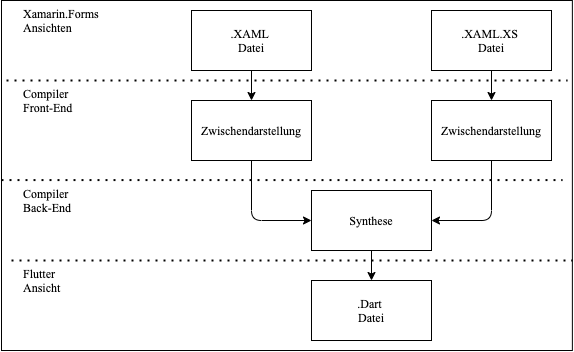
\includegraphics[width=\textwidth,keepaspectratio]{Images/Implementation/ViewCompiler.png}
 \caption{Compiler Phasen für Ansichten}
 \label{fig:ViewCompilerPhases}
\end{figure}

\subsection{Visuellen- Zwischendarstellung}

Für die visuelle Zwischendarstellung wird in einem ersten Schritt die XML Struktur
aus der XAML Datei ausgelesen und ein Syntaxbaum angelegt.  Die entsprechenden Klassen für dessen Behandlung sind in Abbildung \ref{fig:Klassendiagram} in Form eines Klassendiagramms veranschaulicht.

\begin{figure}[!ht]
 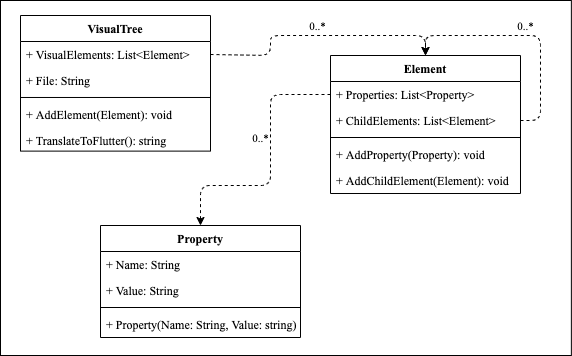
\includegraphics[width=\textwidth,keepaspectratio]{Images/Implementation/Klassendiagram.png}
 \caption{Klassendiagramm}
 \label{fig:Klassendiagram}
\end{figure}

Ein Objekt der Klasse VisualTree stellt den Layout-Baum einer speziellen XAML Datei dar.  Er beinhaltet eine Auflistung von untergeordneten Elementen,  die weitere Elemente beinhalten können,  sodass eine Verschachtlung entsteht.  Jedes Element besitzt eine Auflistung von Eigenschaften, die Attribute der einzelnen XML Knoten beschreiben.  Der Xamarin.Forms Layout- Baum wird,  durch die in Kapitel 4 beschriebenen Repräsentationen von Flutter Widgets, in einen Flutter Widget-Baum überführt und für jedes Widget der Quelltext zur Initialisierung in einem Template vorgehalten.  Alle Eigenschaften besitzen in dieser Vorlage vorgefertigte Platzhalter wie in Quelltext \ref{lst:Placeholder} dargestellt.

\lstinputlisting[label={lst:Placeholder},caption={Flutter Widget Template} , language=Dart]{SourceCode/DartPlaceholder.dart} 

Aufgrund von Inkompatibilitäten zwischen den von Xamarin.Forms gelieferten und von Flutter erwarteten Eigenschaftswerten ist es notwendig diese umzuwandeln.  Der folgende Quelltext \ref{lst:Parsing} zeigt die Umwandlung von Textgrößen.  Xamarin.Forms erwartet diesen Wert entweder als Zahl oder als sogenannte benannte Größe wie Large oder Title,  während Flutter ausschließlich Textgrößen mit dem Typen Double akzeptiert.   

\lstinputlisting[label={lst:Parsing},caption={FontSize Umwandlung} , language=csh]{SourceCode/CSharpFontSize.cs} 

Neben dieser Umwandlung sind auch weitere Anpassungen an weiteren Eigenschaften notwendig.  Dazu zählen unter anderem auch Farben und die Wahl einer Textumbruchoption.  Da die Implementierungen vergleichbar sind,  wird auf diese nicht näher eingegangen. 

Nun erfolgt die Anlage einer Arbeitskopie des Templates,  um in weiteren Compilerphasen die Werte aus der Xamarin.Forms App einzufügen.  Abbildung \ref{fig:PlaceholderOptions} visualisiert, die Behandlung der Platzhalter in den einzelnen Phasen der Übersetzung.

\newpage
\begin{figure}[!ht]
 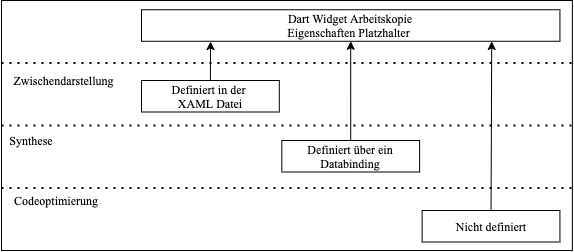
\includegraphics[width=\textwidth,keepaspectratio]{Images/Implementation/DartPlaceHolder.png}
 \caption{Bereinigung von Dart Widget Platzhaltern}
 \label{fig:PlaceholderOptions}
\end{figure}
Es wird deutlich, dass in der Zwischendarstellung ausschließlich XAML definierte Eigenschaftswerte 
importiert werden.  Während der Synthese erfolgt der Austausch der sogenannten Databindings, die den Wert aus der Codebehind-Datei erhalten.  Zur Übersetzung werden neue Platzhalter mit dem Prefix \glq BindingPlaceholder \grq{} benötigt die in der Arbeitskopie hinterlegt sein müssen. Exemplarisch wird in Quelltext  \ref{lst:PlaceholderBinding} der Text-Platzhalter zu einem Binding Platzhalter umgewandelt,  und der Platzhalter textAlign mit einem Wert versehen. 

\lstinputlisting[label={lst:PlaceholderBinding},caption={Flutter Widget mit Binding-Platzhaltern} , language=Dart]{SourceCode/DartPlaceholderBinding.dart} 

Zu diesem Zeitpunkt sind in der Arbeitskopie noch die Binding- und ungenutzten Platzhalter vorhanden.  Diese müssen wie, in der Abbildung \ref{fig:PlaceholderOptions} visualisiert,  in späteren Phasen der Kompilierung entfernt werden.  Grundsätzlich lässt sich aus der XAML ableiten,  welche Platzhalten nicht benötigt werden,  da die Bereinigung jedoch eine Teilaufgabe der Optimierung darstellt wird diese erst in der entsprechenden Phase durchgeführt. 

\subsection{Logische- Zwischendarstellung}

Die Erzeugung der logischen Zwischendarstellung erfordert die gleiche Logik wie die der Klassenstrukturen,  da es sich bei diesen Dateien ebenfalls um \Csharp Klassen handelt.  Während Xamarin.Forms Änderungen an den Eigenschaften automatisch, mithilfe der \glq INotifyPropertyChanged\grq{} Schnittstelle,  an die Benutzeroberfläche übermittelt, muss bei Flutter das Framework mithilfe der \glq setState())\grq{} Methode informiert werden.  Notwendige Änderungen können jedoch nicht im Rahmen der Zwischendarstellungserstellung durchgeführt werden,  da anhand der Codebehind Datei,  nicht identifizierbar ist,  welche Eigenschaft einen direkten Bezug auf die grafische Benutzeroberfläche haben.

\subsection{Visuelle Synthese}

Die Synthese ist eine Teilaufgabe des Compiler Backends und befasst sich mit der Zusammenführung der einzelnen Zwischendarstellungen.  In diesem Falle werden jedoch die visuelle und logische Zwischendarstellung miteinander kombiniert um eine gemeinsame Zwischendarstellung zu generieren.  Die in der nächsten Phase mit den übersetzten Klassenstrukturen zusammengeführt werden kann. 

In einem ersten Schritt erfolgt die Kopie der übersetzen Logik unterhalb der für den Aufbau der grafischen Benutzeroberfläche beinhaltenden Build Methode.  Im nächsten Schritt werden ereignisauslösende Aktivitäten,  beispielsweise der Klick auf Schaltflächen,  mit den übersetzen Methoden verbunden und die Platzhalter entfernt.  Die in der visuellen Zwischendarstellung angelegten Binding Platzhalter geben nun Rückschluss darauf,  welche Eigenschaften Änderungen der der Benutzeroberfläche vornehmen.  Änderungen an diesen müssen folglich mit einem SetState Block umschlossen werden, damit sich die grafische Benutzeroberfläche auch in Flutter aktualisiert. 

Eine Überprüfung welche Eigenschaften der Codebehind-Klassen am Front-End Änderungen durchgeführt haben, wird mittels Binding-Platzhaltern vollzogen.  So müssen alle Bereiche im Quelltext, die Änderungen an Eigenschaften vornehmen zu denen es ein Binding-Placeholder gibt mit einem SetState Block umschlossen werden.

%Quelltext
\section{Ganzheitliche Synthese}
Nach der Generation der Zwischendarstellungen von sowohl Logik und Ansichten müssen diese Darstellungen ebenfalls Synthetisiert werden wo dies notwendig ist.  Nach der Erfolgreichen Übersetzung einer Anwendung sollen Entwickler in der Lage sein die Anwendung wie gewohnt weiter entwickeln zu können.  Dafür ist es notwendig,  abgesehen von dem Codebehind-Datei Konzept,  die selbe Dateistruktur beizubehalten.  In \Csharp wurden diese Dateien wie bereits eingeführt über Namespaces eingebunden.  Da Dart keine Namespaces verwendet sondern Dateien über ihren Namen einbindet ist es notwendig,  diese zu ermitteln.  Die Namespace Information ist dafür nur begrenzt hilfreich,  da ein Namespace über verschiedene Dateien Klassen inkludieren kann.  Daher wird während der Übersetzung analysiert in welcher Datei,  welche Klassen definiert wurden.  Basierend auf dieser Erkenntnis werden in einer späteren Phase bei Verwendung von diesen Klassen Imports zu den Dateien gesetzt.  Diese Referenzen sind ebenfalls wichtig für die Navigation durch die Anwendung,  da Navigationsziele ebenfalls Importiert werden müssen.  Der Compiler geht in diesem Falle davon aus,  das Dateien, die Ansichten beinhalten den gleichen Namen haben wie die Seiten die sie repräsentieren.


\section{Codeoptimierung}

Nach der erfolgreichen Zusammenführung der einzelnen Artefakte kann anschließend der Code optimiert werden.  Dafür werden Sprachkomponenten entfernt,  die ausschließlich für die Arbeit von Xamarin.Forms benötigt sind.  Dazu gehört die \glq InitializeComponent\grq{} Methode,  welche aus der Codebehind-Datei die grafische Benutzeroberfläche lädt und in Flutter nicht benötigt wird.  

Ein weiterer Schritt der Bereinigung das entfernen der \glq INotifyPropertyChangedgrq{} Schnittstellen Definition die in Xamarin.Forms für die Oberflächen- Aktualisierung zuständig ist und bereits durch SetState-Blöcke ersetzt wurde.  Hierfür ist es notwendig,  die Ereignisdefinition, den Ereignis-Handler und alle Aufrufe zu entfernen.

Jetzt folgt die Entfernung der nicht benötigten Platzhalter,  mit dem in Quelltext \ref{lst:PlaceholderCleanup} dargestellten Algorithmus,  aus dem generierten Dart Quelltext.  Damit befindet sich der Programmcode in in einem korrekten syntaktischen Zustand und kann mit Hilfe des Flutter Compilers zu einer mobilen App übersetzt und ausgeführt werden. 
\newpage
\lstinputlisting[label={lst:PlaceholderCleanup},caption={Bereinigung von ungenutzten Platzhaltern}, language=csh]{SourceCode/Cleanup.cs}


\section{Grafische Benutzeroberfläche}
Die GUI ist der zentrale Berührungspunkt von Anwendern mit dem Transpiler.  Sie soll die notwendigen Eingabe-Möglichkeiten anbieten, das Ergebnis ausgeben und den Anwender auf mögliche Fehler hinweisen.  Das grafische Vorbild ist das in Kapitel 3 entworfene Mockup, siehe Abbildung 3.4.  Für die Erstellung einer entsprechenden Benutzeroberfläche stehen eine Vielzahl von Technologien mit verschiedenen Vor- und Nachteilen zur Verfügung. Eine Webseite erspart dem Anwender einen hohen Installationsaufwand und ermöglicht die plattformunabhängige Verwendung des Compilers.  Allerdings ist zumindest ein gewisser Kontrollverlust über den eigenen Quelltext durch das  Hochladen auf eine Webseite nicht ausgeschlossen.  Die Bedienoberfläche dieser Arbeit soll daher eine lokale Anwendung sein, sodass kein  unberechtigter Zugriff auf den Source-Code möglich ist.  Zu diesem Zweck wird die GUI mit der Technologie \ac{wpf} realisiert.  Dabei handelt es sich um ein UI-Framework des .NET Frameworks, das für die Erstellung von Desktopanwendungen geeignet ist die mit XAML und \Csharp entwickelt werden. \footcite[Vgl.][S. 1f]{Wenger2012} 

Anwendungen die mittels WPF programmiert werden, sind nur unter Windows als Betriebssystem ausführbar.  Da der Roslyn Compiler auch nur unter Windows verfügbar ist entstehen hier keine zusätzlichen Einschränkungen.  Die folgende Darstellung \ref{fig:CompilerUI} zeigt das Erscheinungsbild der Anwendung nach einer erfolgreichen Übersetzung.

\begin{figure}[!ht]
 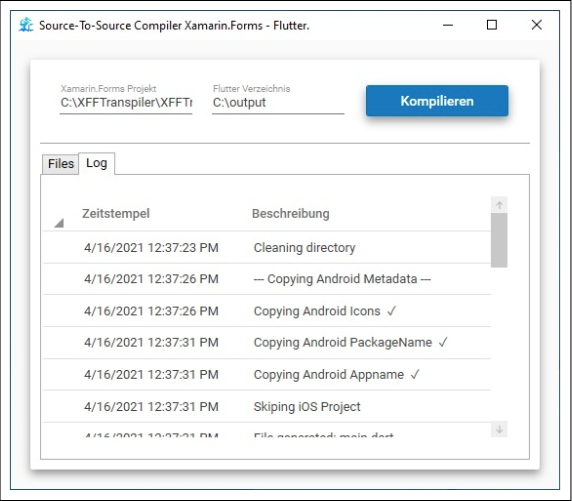
\includegraphics[width=\textwidth,keepaspectratio]{Images/Implementation/UiScreenshot.png}
 \caption{Grafische Oberfläche des Compilers}
 \label{fig:CompilerUI}
\end{figure}

Wie die Ansicht veranschaulicht, werden die durchgeführten Arbeitsschritt durch Log-Einträge in der Anwendung angezeigt.
Die Realisierung der grafischen Benutzeroberfläche als auch des Source-To-Source Compilers erfolgte mit  .Net Technologien,  sodass es möglich ist den Compiler als Abhängigkeit in das Projekt der grafischen Benutzeroberfläche zu laden und von dort aus die Übersetzung zu starten.  


